% !TEX TS-program = pdflatex
% !TEX encoding = UTF-8 Unicode

% This is a simple template for a LaTeX document using the "article" class.
% See "book", "report", "letter" for other types of document.

\documentclass[11pt]{article} % use larger type; default would be 10pt

\usepackage[utf8]{inputenc} % set input encoding (not needed with XeLaTeX)

%%% Examples of Article customizations
% These packages are optional, depending whether you want the features they provide.
% See the LaTeX Companion or other references for full information.

%%% PAGE DIMENSIONS
\usepackage{geometry} % to change the page dimensions
\geometry{a4paper,margin=0.5in} % or letterpaper (US) or a5paper or....
 %\geometry{margins=2in}{a4paper} % for example, change the margins to 2 inches all round
% \geometry{landscape} % set up the page for landscape
%   read geometry.pdf for detailed page layout information

\usepackage{graphicx} % support the \includegraphics command and options

% \usepackage[parfill]{parskip} % Activate to begin paragraphs with an empty line rather than an indent
\usepackage{graphicx}
\usepackage{caption}
\usepackage{color} 
\usepackage{epstopdf}
\usepackage{rotating}
\usepackage{lscape}
\usepackage{lineno}
\usepackage{multirow}
%%% PACKAGES
\usepackage{amsmath} 
\usepackage[table]{xcolor}
\usepackage{breakcites}
\usepackage{amsfonts}
\usepackage{booktabs} % for much better looking tables
\usepackage{array} % for better arrays (eg matrices) in maths
\usepackage{paralist} % very flexible & customisable lists (eg. enumerate/itemize, etc.)
\usepackage{verbatim} % adds environment for commenting out blocks of text & for better verbatim
\usepackage{subfig}
% make it possible to include more than one captioned figure/table in a single float
% These packages are all incorporated in the memoir class to one degree or another...
\usepackage{bm}
%%% HEADERS & FOOTERS
\usepackage{fancyhdr} % This should be set AFTER setting up the page geometry

\usepackage{authblk}

\pagestyle{fancy} % options: empty , plain , fancy
\renewcommand{\headrulewidth}{0pt} % customise the layout...
\lhead{}\chead{}\rhead{}
\lfoot{}\cfoot{\thepage}\rfoot{}

%%% SECTION TITLE APPEARANCE
\usepackage{sectsty}
\allsectionsfont{\sffamily\mdseries\upshape} % (See the fntguide.pdf for font help)
% (This matches ConTeXt defaults)

%%% ToC (table of contents) APPEARANCE
\usepackage[nottoc,notlof,notlot]{tocbibind} % Put the bibliography in the ToC
\usepackage[titles,subfigure]{tocloft} % Alter the style of the Table of Contents
\renewcommand{\cftsecfont}{\rmfamily\mdseries\upshape}
\renewcommand{\cftsecpagefont}{\rmfamily\mdseries\upshape} % No bold!
%%% END Article customizations

%%% The "real" document content comes below...

\title{Supervised Learning in Spiking Neural Networks with FORCE Training} 


\date{\today} % Activate to display a given date or no date (if empty),
         % otherwise the current date is printed 
\author[1]{Wilten Nicola}
\author[1]{Claudia Clopath \thanks{c.clopath@imperial.ac.uk}}
\affil[1]{Department of Bioengineering, Imperial College London.  Royal School of Mines\\ London  UK\\  SW7 2AZ}

\begin{document}
\maketitle    


\section*{Acceptance} Note that this manuscript has been accepted and published as of Dec 20th, 
2017 in Nature Communications.  Please cite the following when referencing this manuscript: 


\textbf{
Nicola, W., \& Clopath, C. (2017). Supervised learning in spiking neural networks with FORCE training. Nature communications, 8(1), 2208.}


\section*{Abstract}

Populations of neurons display an extraordinary diversity in the behaviors they affect and display. 
Machine learning techniques have recently emerged that allow us to create networks of model neurons 
that display behaviours of similar complexity. Here, we demonstrate the direct applicability of one 
such technique, the FORCE method, to spiking neural networks.  We train these networks to mimic 
dynamical systems, classify inputs, and store discrete sequences that correspond to the notes of a song. 
Finally, we use FORCE training to create two biologically motivated model circuits. One is inspired by the  
zebra-finch and successfully reproduces songbird singing. The second network is motivated by the hippocampus 
and is trained to store and replay a movie scene.   
FORCE trained networks reproduce behaviors comparable in complexity to their inspired circuits and 
yield information not easily obtainable with other techniques such as behavioral responses to 
pharmacological manipulations and spike timing statistics.  

\section*{Introduction}  

Human beings can naturally learn to perform a wide variety of tasks  quickly and efficiently.  
Examples include learning the complicated sequence of motions in order to take a slap-shot in Hockey or 
learning to replay the notes of a song after music class.   
While there are approaches to solving these different problems in fields such as machine learning, 
control theory, etc., humans use a very distinct tool to solve these problems: the spiking neural network.  

Recently, a broad class of techniques have been derived that allow us to enforce a certain behavior or 
dynamics onto a neural network \cite{FORCE1,FORCE2,FORCE3,FORCE4,Deneve1,Deneve2,Deneve4,Chris1,Chris2,Gilra}.  
These top-down techniques start with an intended task that a recurrent spiking neural network should perform, 
and determine what the connection strengths between neurons should be to achieve this.   
The dominant approaches are currently the FORCE method \cite{FORCE1,FORCE2},  spike-based or 
predictive coding networks \cite{Deneve1,Deneve2,Deneve4}, and the 
Neural Engineering Framework (NEF) \cite{Chris1,Chris2}.  Both the NEF and spike-based coding approaches 
have yielded substantial insights into network functioning.  
Examples include how networks can be organized to solve behavioral problems \cite{Chris1} 
or process information in robust but metabolically efficient ways \cite{Deneve1,Deneve2}.  


\section*{Results} 

\subsection*{FORCE Training Weight Matrices} 

We explored the potential of the FORCE method in training spiking neural networks to perform an arbitrary task.  
In these networks, the synaptic weight matrix is the sum of a set of static weights and a 
set of learned weights $\bm \omega = G\bm{\omega}^0+Q\bm \eta \bm \phi^T$.   
The static weights, $G\bm\omega^0$ are set to initialize the network into 
chaotic spiking  \cite{SOMP,OSTOJIC,Harish}.  The learned component of the weights, $\bm \phi$, 
are determined online using a supervised learning method called Recursive Least Squares (RLS).  
The quantity $\bm \phi$ also serves as a linear decoder for the network dynamics.  
The parameter $\bm \eta$ defines the tuning preferences of the neurons to the learned feedback term.  
The components of $\bm\eta$ are static and always randomly drawn.  
The parameters $G$ and $Q$ control the relative balance between the chaos inducing static 
weight matrix and the learned feedback term, respectively.  The parameters are discussed in 
greater detail in the Materials and Methods. The goal of RLS is to minimize the squared error 
between the network dynamics ($\hat{x}(t)$) and the target dynamics (i.e. the task, $x(t)$) 
(Figure \ref{FORCE1}A) \cite{haykin,bishop}.  
This method is successful if the network dynamics can mimic the target dynamics when RLS is turned off.   
We considered three types of spiking integrate-and-fire model: the theta model, the leaky 
integrate-and-fire (LIF) and the Izhikevich model (see Materials and Methods for a more detailed explanation).  
The parameters for the models can be found in Table \ref{Table1}.  
All networks considered were constrained to be intermediate in size (1000-5000 neurons), 
have low post-training average firing rates ($<60$ Hz).  
The synaptic time constants were typically $\tau_R = 2$ ms and $\tau_D$ = 20 ms with other values 
considered in the Supplementary Material.   
The code used for this paper can be found on modelDB (\cite{modeldb}), under accession number 190565.


\subsubsection*{FORCE Trained Rate Networks Learn Using Chaos} 

To demonstrate the basic principle of this method and to compare with our spiking network simulations, 
we applied FORCE training to a network of rate equations (Figure \ref{FORCE1}A) as in \cite{FORCE1}.  
We trained a network to learn a simple 5 Hz sinusoidal oscillator.  
The static weight matrix initializes high-dimensional chaotic dynamics onto the network of rate equations 
(Figure \ref{FORCE1}B).  These dynamics form a suitable reservoir to allow the network to learn from a 
target signal quickly.   As in the original formulation of the FORCE method, the rates are 
heterogeneous across the network and varied strongly in time (see Figure 2A in \cite{FORCE1}). 
RLS is activated after a short initialization period for the network.  
After learning the appropriate weights $\phi_j $ (Figure \ref{FORCE1} D), 
the network reproduces the oscillation without any guidance from the teacher signal, 
albeit with a slight frequency and amplitude error (Figure \ref{FORCE1}C).   
To ascertain how these networks can learn to perform the target dynamics, 
we computed the eigenvalues of the resulting weight matrix before and after learning 
(Figure \ref{FORCE1}E).  Unlike other top-down techniques, FORCE trained weight matrices are always 
high rank \cite{AbbottR}, and as we will demonstrate, can have dominant eigenvalues for large $Q$.


\subsection*{High-Dimensional Temporal Signals Improve FORCE Training}

We were surprised at how robust the performance of the songbird network was given 
the high dimensionality and complicated structure of the output.  
We hypothesized that the performance of this network was strongly associated to the precise, 
clock-like inputs provided by HVC and that similar inputs could aid in the encoding and 
replay of other types of information.  To test this hypothesis, we removed the HVC input pattern 
and found that the replay of the learned song was destroyed (not shown), 
similar to experimental lesioning of this area in adult canaries \cite{nottebohm}.   
Due to the temporal information that these high-dimensional signals provide, 
we will subsequently refer to them as High-Dimensional Temporal Signals 
(HDTS, See Materials and Methods for further details).   

To further explore the benefits that an HDTS might provide, we FORCE trained a network of 
Izhikevich neurons to internally generate its own HDTS, while simultaneously also training 
it to reproduce the first bar of Ode to Joy.  
The entire supervisor consisted of the 5 notes used in the first bar of the song, 
in addition to 16 other components.  These correspond to a sequence of 16 pulses that partition time.  
The network learned both the HDTS and the song simultaneously, 
with less training time, and greater accuracy than without the HDTS.  
As the HDTS helped in learning and replaying the first bar of a song, 
we wondered if these signals could help in encoding longer sequences.  
To test this hypothesis, we FORCE trained a network to learn the first four bars of Ode to Joy, 
corresponding to a 16 second song in addition to its own, 64-dimensional HDTS.  
The network successfully learned the song post-training, without any error in the sequence of 
notes in spite of the length and complexity of the sequence (see Supplementary Fig. 17, Supplementary Movie 2).  
Thus, an internally generated HDTS can make FORCE training faster, more accurate, 
and more robust to learning longer signals.  We refer to these networks as having 
an internally generated HDTS.    



\section*{Discussion} 

We have shown that FORCE training can take initially chaotic networks of 
spiking neurons and use them to mimic the natural tasks and functions demonstrated 
by populations of neurons.  For example, these networks were trained to learn 
low-dimensional dynamical systems such as oscillators which are at the heart of 
generating both rhythmic and non rhythmic motion \cite{CHURCHLAND1}.   
We found FORCE training to be robust to the spiking model employed, 
initial network states, and synaptic connection types.   

Additionally, we showed that we could train spiking networks to display behaviors 
beyond low dimensional dynamics by altering the supervisor used to train the network.  
For example, we trained a statistical classifier with a network of Izhikevich neurons 
that could discriminate its inputs.  
Extending the notion of an oscillator even further allowed us to store a complicated 
sequence in the form of the notes of a song, reproduce the singing behavior of songbirds, 
and encode and replay a movie scene. 
These tasks are aided by the inclusion of a high-dimensional temporal signal (HDTS) 
that discretizes time by segregating the neurons into assemblies.  
 

Top-down network training techniques have different strengths and uses.   
For example, the Neural Engineering Framework (NEF) and spike-based coding 
approaches solve for the underlying weight matrices immediately without 
training \cite{Deneve1,Deneve2,Ali,Chris1,Chris2}.  
The solutions can be analytical as in the spike based coding approach, 
or numerical, as in the NEF approach.  Furthermore, the weight matrix solutions 
are valid over entire regions of the phase space, where as FORCE training uses individual 
trajectories as supervisors.  
Multiple trajectories have to be FORCE trained into a single network to yield a 
comparable level of global performance over a region.   
Both sets of solutions yield different insights into the structure, dynamics, 
and functions of spiking neural networks.  
For example, brain scale functional models can be constructed with 
NEF networks \cite{Chris1}.  Spike-based coding networks demonstrate 
how higher order error scaling is possible by utilizing spiking sparsely and 
efficiently through balanced network solutions.  
While the NEF and spike based coding approaches provide immediate 
weight matrix solutions, both techniques are difficult to generalize 
to other types of networks or other types of tasks.  
Both the NEF and spike based coding approach require a system of closed 
form differential equations to determine the static weight matrix 
that yields the target dynamics.  

In summary, we showed that FORCE can be used to train spiking 
neural networks to reproduce complex spatio-temporal dynamics. 
This method could be used in the future to mechanically link neural 
activity to the complex behaviors of animals.

\renewcommand{\abstractname}{Acknowledgements}
\begin{abstract}
This work was funded by a Canadian National Sciences and 
Engineering Research Council (NSERC) Post-doctoral Fellowship, 
by the Wellcome Trust (200790/Z/16/Z), the Leverhulme Trust (RPG-2015-171) 
and the BBSRC (BB/N013956/1 and BB/N019008/1).  
We would like to thank Frances Skinner, Chris Eliasmith, Larry Abbott, 
Raoul-Martin Memmesheimer, Brian DePasquale and Dean Buonomano for their comments.  
Finally, we would like to especially thank the anonymous referees.  
Their comments and suggestions greatly improved this manuscript. 
\end{abstract}

\renewcommand{\abstractname}{Conflict of Interest} 
\begin{abstract}
There is no conflict of interest to declare.   
\end{abstract}

\renewcommand{\abstractname}{Author Contributions}
\begin{abstract}
WN performed wrote software and performed simualtions.  
Investigation and analysis was performend by WN and CC.  
WN and CC wrote the manuscript.   
\end{abstract}


\renewcommand{\abstractname}{Data Availability Statement}
\begin{abstract}
The code used for this paper can be found on modelDB (\cite{modeldb}), 
under accession number 190565.
\end{abstract}

\section*{Methods} 
\subsection*{Rate Equations} 

The network of rate equations is given by the following:
\begin{eqnarray}
\tau_s\dot{s}_i &=& -s_i + G\sum_{j=1}^N \omega^0_{ij} r_j + Q\eta_i \hat{x}\\
r_j &=& \begin{cases} F \sqrt{s_j} & s_j\geq 0 \\ 0 & s_j <0   \end{cases} \\
\hat{x}(t) &=& \sum_{j=1}^N \phi_j r_j(t) 
\end{eqnarray} 
where $\omega^0_{ij} $ is the sparse and static weight matrix that induces 
chaos in the network by having $\omega^0_{ij}$ drawn from a normal distribution 
with mean 0 and variance $(Np)^{-1}$, where $p$ is the degree of sparsity 
in the network.  The variables $s$ can be thought of as neuronal 
currents with a postsynaptic filtering time constant of $\tau_s$.   
The encoding variables $\eta_i$ are drawn from a uniform distribution 
over $[-1,1]$ and set the neurons encoding preference over the phase space 
of $x(t)$, the target dynamics.  The quantities $G$ and $Q$ are constants 
that scale the static weight matrix and feedback term, respectively.   
The firing rates are given by $r_j$ and correspond to the Type-I normal form for firing.  
The variable $F$ scales the firing rates.    
The decoders, $\phi_j$ are determined by the Recursive Least Mean Squares (RLS) technique, 
iteratively \cite{haykin,bishop}.  RLS is described in greater detail in the next section.  
For Supplementary Fig. 8 and Supplementary Fig. 9, 
we also implemented the $tanh(x)$ continuous variable equations 
from \cite{FORCE1} for comparison purposes.  
These equations are described in greater detail in \cite{FORCE1}.  
 



\subsection*{Integrate-and-Fire Networks} 
Our networks consist of coupled integrate-and-fire neurons, 
that are one of the following three forms: 
\begin{eqnarray}
\dot{\theta}_i &=& (1-\cos(\theta_i)) +\pi^2 (1+\cos(\theta_i))( I)  \quad \text{(Theta neuron)}\\
\tau_m\dot{v}_i &=& -v_i + I  \quad \text{(LIF Neuron)} \\
C\dot{v}_i &=& k(v_i-v_r)(v_i-v_t) - u_i +I  \quad \text{(Izhikevich Neuron)} \\
\dot{u}_i &=& a(b(v_i -v_r) - u_i) 
\end{eqnarray}

The currents, $I$ are given by $I=I_{Bias}+ s_i$ where $I_{Bias}$ is a constant background current 
set near or at the rheobase (threshold to spiking) value.   
The currents are dimensionless in the case of the theta neuron while dimensional for the LIF and Izhikevich models.  
Note that we have absorbed a unit resistance into the current for the LIF model.   
The quantities $\theta_i$, or $v_i$ are the voltage variables while $u_i$ is the 
adaptation current for the Izhikevich model.  
These voltage variables are instantly set to a reset potential ($v_{reset}$) when a 
neurons membrane potential reaches a threshold ($v_{thr}$,LIF) or voltage peak 
($v_{peak}$, theta model, Izhikevich model).  The parameters for the neuron models 
can be found in Table \ref{Table1}.  The parameters from the Izhikevich model are from \cite{ahmad} 
with a slight modification to the $k$ parameter.  The LIF model has a refractory time period, 
$\tau_{ref}$ where the neuron cannot spike.      
The adaptation current, $u_i$ for the Izhikevich model increases by a discrete amount 
$d$ every time neuron $i$ fires a spike and serves to slow down the firing rate.  
The membrane time constant for the LIF model is given by $\tau_m$.  
The variables for the Izhikevich model include $C$ (membrane capacitance), 
$v_r$ (resting membrane potential), $v_t$ (membrane threshold potential), 
$a$ (reciprocal of the adaptation time constant), 
$k$ (controls action potential half-width) and $b$ (controls resonance properties of the model).  

The spikes are filtered by specific synapse types.  
For example, the single exponential synaptic filter is given by the following:
\begin{eqnarray}
\dot{r}_j = -\frac{r_j}{\tau_s} + \frac{1}{\tau_s}\sum_{t_{jk}<t}\delta(t-t_{jk})  \label{fr11}
\end{eqnarray}
where $\tau_s$ is the synaptic time constant for the filter and $t_{jk}$ 
is the $k$th spike fired by the $j$th neuron.  
The double exponential filter is given by 
\begin{eqnarray}
\dot{r}_j &=& -\frac{r_j}{\tau_d} + h_j \\
\dot{h}_j&=& -\frac{h_j}{\tau_r} + \frac{1}{\tau_r\tau_d} \sum_{t_{jk}<t}\delta(t-t_{jk})  \label{fr12}
\end{eqnarray}
where $\tau_r$ is the synaptic rise time, and $\tau_d$ is the synaptic decay time.    
The filters can be of the simple exponential type, double exponential, 
or alpha synapse type ($\tau_r = \tau_d$).   
However, we will primarily consider the double exponential filter with a rise time of 
2 ms and a decay time of 20 ms.  
Longer and shorter filters are considered in the Supplementary Materials.   

The synaptic currents, $s_i(t)$, are given by the equation 
\begin{eqnarray}
s_i = \sum_{j=1}^N  \omega_{ij}r_j 
\end{eqnarray} 
The matrix $\omega_{ij}$ is the matrix of synaptic connections and controls 
the magnitude of the postsynaptic currents arriving at neuron $i$ from neuron $j$.  

 The primary goal of the network is to approximate the dynamics of an 
$m$-dimensional teaching signal, $\bm x(t)$, with the following approximant:
\begin{eqnarray}
\hat{\bm{x}}(t) = \sum_{j=1}^N \bm \phi_j r_j
\end{eqnarray}
where $\bm \phi_j$ is a quantity that is commonly referred to as the 
linear decoder for the firing rate.   
The FORCE method decomposes the weight matrix into a static component, 
and a learned decoder $ \bm{\phi}$:
\begin{eqnarray}
\omega_{ij} = G \omega^0_{ij} + Q \bm{\eta}_i \cdot \bm{\phi}_j  ^T
\end{eqnarray}
The sparse matrix $\omega_{ij}^0$ is the static weight matrix that induces chaos.  
It is drawn from a normal distribution with mean $0$, and variance $(Np^2)^{-1}$, 
where $p$ is the sparsity of the matrix.  Additionally, the sample mean for 
these weight matrices was explicitly set to $0$ for the LIF and theta neuron 
models to counterbalance the resulting firing rate heterogeneity.  
This was not necessary with the Izhikevich model.   
The variable $G$ controls the chaotic behavior and its value varies from 
neuron model to neuron model.   The encoding variables, $\bm \eta_i$ are 
drawn randomly and uniformly from $[-1,1]^k$, where $k$ is the dimensionality of 
the teaching signal.  The encoders, $\bm \eta_i$, contribute to the tuning 
preferences of the neurons in the network.  The variable $Q$ is increased 
to better allow the desired recurrent dynamics to tame the chaos present in the reservoir.    
The weights are determined dynamically through time by minimizing 
the squared error between the approximant and intended dynamics, 
$\bm{e}(t) = \hat{\bm{x}}(t) -\bm{x}(t)$.  
The Recursive Least Squares (RLS) technique updates the decoders accordingly:
\begin{eqnarray}
\bm{\phi}(t) &=& \bm{\phi}(t-\Delta t) - \bm{e}(t)\bm{P}(t)\bm{r}(t) \label{eq14} \\
\bm{P}(t) &=& \bm{P}(t-\Delta t) -\frac{ \bm{P}(t-\Delta t) \bm{r}(t)\bm{r}(t)^T \bm{P}(t-\Delta t)}{1 + \bm{r}(t)^T \bm{P}(t-\Delta t) \bm{r}(t)} \label{eq15}
\end{eqnarray} 
where $\bm{P}(t)$ is the network estimate for the inverse of the correlation matrix:
\begin{eqnarray}
\bm{P}(t)^{-1} = \int_{0}^t \bm r(t) \bm r(t)^T \,dt + \lambda I_N .
\end{eqnarray}
The parameter $\lambda$ acts both as a regularization parameter \cite{haykin} 
and controls the rate of the error reduction while $I_N$ is an $N\times N$ identity matrix.  
The RLS technique can be seen to minimize the squared error between 
the target dynamics and the network approximant:
\begin{eqnarray}
C = \int_0^T(\hat{x}(t)-x(t))^2\,dt + \lambda \bm{\phi}^T \bm{\phi}  
\end{eqnarray}
and uses network generated correlations optimally by using the correlation matrix $P(t)$.  
The network is initialized with $\bm{\phi}(0) = \bm 0$, $\bm P(0) = I_N\lambda^{-1}$, 
where $I_N$ is an $N$-dimensional identity matrix.  
Note that in the original implementation of \cite{FORCE1}, 
equation (\ref{eq14}) contains the term $1+\bm r(t)^T \bm P(t-\Delta t) \bm r(t)$ in the denominator.  
This term adds a slight increase in accuracy and stability, but does not change 
the overall order of convergence of RLS.  
For comparison purposes, this modification was applied to Supplementary Fig. 8.  
All other implementations used equations (\ref{eq14})-(\ref{eq15}).   

\subsubsection*{$G$ and $Q$ parameters}  

In \cite{FORCE1}, the learned recurrent component and the static feedback term 
were both of the same order of magnitude, $O(1)$.  
Furthermore, if the input stimulus had an amplitude that was too small 
(see Figure 2K, \cite{FORCE1}), the chaotic dynamics could not be tamed.  
Operating on the hypothesis that the static term and the learned term require 
fluctuations of the same order of magnitude, one can derive the following 
equations using standard arguments about balanced networks \cite{sompo1}:
\begin{eqnarray}
s_i(t)&=&\sum_{j=1}^N G\omega_{ij}^0 r_j(t) \\
\langle s_i(t) \rangle &\sim& 0, \quad N\rightarrow \infty\\
\langle s_i(t)^2\rangle & \sim & G^2 E((\bar{\omega}_{ij}^0)^2) \langle r_i(t)^2\rangle 
\end{eqnarray}
where $\bar{\omega_{ij}}^0 = \sqrt{N} \omega_{ij}^0$
The second term can be derived as follows:
\begin{eqnarray}
s_i(t)^2 &=&\frac{ G^2}{N}\left( \sum_{j=1}^N (\bar{\omega}_{ij}^0)^2 r_j(t)^2 + \sum_{j\neq k}b\bar{\omega_{ij}^0}\bar{\omega_{ik}^0} r_j(t)r_k(t)   \right)\\
&\sim & {G^2} E((\bar{\omega}^0_{ij})^2)\langle r_{j}(t)^2\rangle \quad N\rightarrow \infty  
\end{eqnarray}
where the last step is justified as we can ignore interneuronal correlations 
$r_i(t)r_j(t)$ in addition to correlations between a weight matrix component 
and a firing rate, $r_j(t)$ in the large network limit.   
If the term $\bm \eta \cdot x(t)$ is $O(1)$, this implies that 
$Q = O({G} \sigma_{\omega} \sqrt{\langle r_{j}(t)^2\rangle})$ where 
$\sigma_\omega$ is the standard deviation of the zero mean, 
static weight matrix distribution. 

\subsection*{High Dimensional Temporal Signals} 

The High-Dimensional Temporal Signals (HDTS) serves to stabilize 
network dynamics by organizing the neurons into assemblies.  
These assemblies fire at precise intervals of time.   
To elaborate further, these signals are constructed as a 
discretization of time, $T$ into $m$ sub-intervals.   
Each subinterval generates an extra component (dimension) in the supervisor 
and within the subinterval, a pulse or upward deflection of the 
supervisor is generated.  For example, if we consider the interval 
from $[0,T]$ with $m$ subintervals of width 
$I_n = [T\left(\frac{n-1}{m}\right),T\left(\frac{n}{m}\right)]$, $n=1,2,\ldots m$.  
The supervisor is constructed as a series of pulses centered in the intervals $I_n$.  
This can be done in multiple ways.  For example, Gaussian pulses 
can be used to construct the HDTS:
\begin{eqnarray}
x_n(t) = \exp\left(-\frac{\left(t - T\left(\frac{2n-1}{2m} \right)\right)^2}{\sigma^2} \right)
\end{eqnarray}
where $\sigma$ controls the width.  Alternatively, 
one can also use piecewise defined functions such as
\begin{eqnarray}
x_n(t) = \begin{cases} |\sin(\frac{m\pi t}{T})| & t\in I_n\\ 0 & \text{otherwise}. \end{cases}
\end{eqnarray}
The end effect of these signals is to divide the network into a series of assemblies.  
A neurons participation in the $n$th assembly is a function of the static weight matrix, 
in addition to $\bm \eta_{in}$.  Each assembly is activated by the preceding assemblies 
to propagate a long signal through the network.  The assemblies are activated at a specific 
frequency in the network, dictated by the width of the pulses in the HDTS.  
Sinusoidal HDTS were used for the all figures with the exception of Supplementary 
Fig. 18C, where a Gaussian HDTS was used.    



\subsection*{The FORCE Method with Rate Networks (Figure 1) }
A network of rate equations is used to learn the dynamics of a teaching signal, $x(t)$, 
a 5 Hz sinusoidal oscillation.  The network consists of 1000 rate neurons with $F = 10$, 
$\tau_s = 10$ ms, $G=1$, and $Q=1.5$, $p=0.1$.    
The network is run for 1 second initially, with RLS run for the next 4 seconds, 
and shut off at the 5 second mark.  The network is subsequently run for another 5 seconds 
to ensure learning occurs.   The smooth firing rates of the network were less than 30 Hz.  
The RLS parameters were taken to be $\Delta t = 2$ ms and $\lambda^{-1} =  0.5$ ms.  

\subsection*{Using Spiking Neural Networks to Mimic Dynamics Using FORCE training (Figure 2)} 

Networks of theta neurons were trained to reproduce different oscillators.  
The parameters were: $N=2000$, $G=10$ (sinusoid, sawtooth), $G = 15$ (Van der Pol), 
$G=25$ (product of sinusoids), $G=15$ (product of sinusoids with noise), $Q = 10^4$, 
$\Delta t = 0.5$ ms, with an integration time step of $0.01$ ms.   
The resulting average firing rates for the network were 26.1 Hz (sinusoid) 29.0 Hz (sawtooth), 
15.0 Hz (Van der Pol relaxation), 18.8 Hz (Van der Pol Harmonic), 23.0 Hz (product of sinusoids), 
21.1 Hz (product of sines with noise). The Van der Pol oscillator is given by: 
$\ddot{x}  = \mu(1-x^2)\dot{x} - x$ for $\mu = 0.3$ (harmonic) and $\mu = 5$ (relaxation)  
and was rescaled in space to lie within $[-1,1]^2$  and sped up in time by a factor of 20.    
The networks were initialized with the static matrix with 10\% connectivity.  
This induces chaotic spiking in the network.  We allow the network to settle onto the 
chaotic attractor for a period of 5 seconds.  After this initial period,  
RLS is activated to turn on FORCE training for a duration of 5 seconds.  
After this period of time, RLS was deactivated for the remainder 5 seconds of simulation time 
for all teaching signals except signals that were the product of sinusoids.  
These signals required 50 seconds of training time and were tested for a longer duration 
post training to determine convergence.   The $\lambda^{-1}$ parameter used for RLS 
was taken to be the integration time step, $0.01$ ms for all implementations of 
the theta model in Figure 2.  The integration time step used in all cases of the 
theta model was $0.01$ ms.  

The theta neuron parameters were as in Figure 2B for the 5Hz sinusoidal oscillator.  
The LIF network consisted of 2000 neurons with $G=0.04$, $Q = 10$, with 10\% 
connectivity in the static weight matrix and $\Delta t = 2.5$ ms with an integration 
time step of 0.5 ms.  The average firing rate was 22.9 Hz.   
The Izhikevich network consisted of 2000 neurons with $G =5*10^3 $, $Q = 5*10^3$, 
with 10\% connectivity in the static weight matrix and $\Delta t =  0.8 $ ms 
and an average firing rate of 36.7 Hz.  The $\lambda^{-1}$ parameter used for RLS 
was taken to be a small fraction of the integration time step, $\lambda^{-1} = 0.0025$ 
ms for Figure 2 while the Izhikevich model had $\lambda^{-1} = 1$ ms and 
an integration time step of $0.04$ ms.    The training time for all networks 
considered was 4 seconds, followed by 5 seconds of testing.  

The Lorenz system with the parameter $\rho = 28$, $\sigma = 10$, and $B=8/3$ 
was used to train a network of 5000 theta neurons and is given by the equations:
\begin{eqnarray*}
\dot{x} &=& \sigma(y-x)\\
\dot{y} &=& x(\rho - z) -y \\
\dot{z} &=& xy -B z.
\end{eqnarray*}
The connectivity parameters were $G=14$, and $Q=10^4$.  
The average firing rate was 22.21 Hz.  The network was trained for 45 seconds, 
and reproduced Lorenz-like trajectories and the attractor for the remaining 50 seconds. 






\subsection*{Using Spiking Neural Networks for Pattern Storage and Replay 
with the FORCE Method: Movie Replay (Figure 5)}

The teaching signal consisted of an 8 second movie clip from the movie Predator.  
The frames were smoothed and interpolated so that RLS could be applied at any time point, 
instead of just the fixed times corresponding to the native frames 
per second of the original movie clip.  The movie was downsampled to 
1920 pixels ($30\times 64$) which formed the supervisor.  
For both implementations (external and internal HDTS), the replay network consisted 
of 1000 neurons with $G=5*10^3$, $Q = 4*10^2$, $\lambda^{-1} =  2$ ms, 
$\Delta t = 4$ ms and an integration time step of $0.04$ ms.  
For the external HDTS network, an HDTS was generated with 32 pulses that 
were 250 ms in duration.  The HDTS was multiplied by a static, $N\times 32$ 
feedforward weight matrix, $W^{in}$ where each weight was drawn uniformly 
from $[-4*10^3,4*10^3]$ and 74 seconds of FORCE training was used.  
The network was simulated for another 370 s after RLS was turned off to test 
if learning was successful.  For the internal HDTS case, a separate 
HDTS network was trained with 2000 neurons.  The supervisor for this network 
consisted of a 64-dimensional HDTS with pulses that were 125 ms in duration.  
The HDTS was fed into an identical replay network as in the external HDTS case.  
The replay network was trained simultaneously to the HDTS network and 
had $G = 1*10^4$, $Q = 4*10^3$.  The HDTS was fed into the replay network 
in an identical manner to the external HDTS case.  RLS was applied to train 
the HDTS and replay network with identical parameters as in the external 
HDTS case, only with a longer training time (290 s).   We note that for this 
movie example, the network could also learn the output with only the static, 
chaos inducing weight matrix and the feedforward HDTS inputs ($Q=0$).  
However when $Q=0$, the network behavior is similar to the more classic 
liquid state regime.  

\newpage

\begin{figure}[htp!]
\centering 
\end{figure}


\begin{figure}[htp!]
\centering
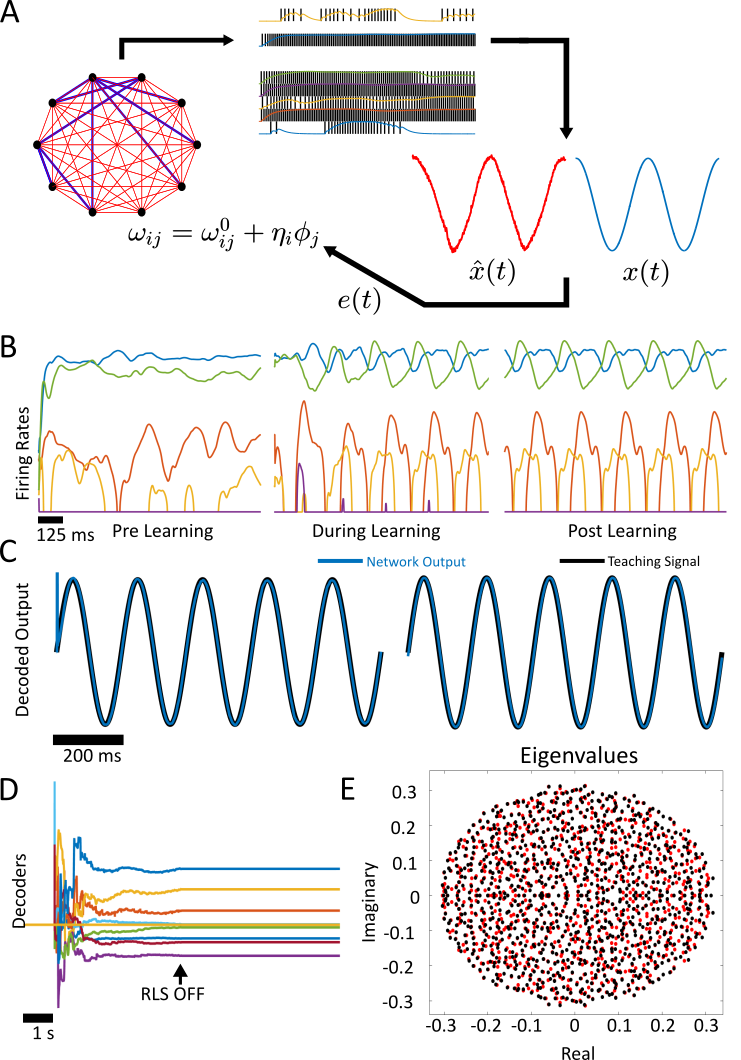
\includegraphics[scale=0.8]{FFIG1}
\caption{}\label{FORCE1}
\end{figure}


\begin{table}[htp!]
\center
\begin{tabular}{|l|l|l|}
\hline 
Neuron Model & Parameter & Value \\
\hline
Izhikevich & $C$ & 250 $\mu$ F  \\ 
\hline
& $v_r$ & -60 mV \\ 
\hline
& $v_{t}$ & -20 mV( -40 mV songbird example, -19.2 mV Supplementary Oscillator Panel) \\ 
\hline
& $b$ & 0  (-2 nS in Supplementary Oscillator Panel)\\ 
\hline
& $v_{peak}$ & 30 mV \\ 
\hline
& $v_{reset}$ & -65 mV \\ 
\hline
& $a$ & 0.01 ms$^{-1}$ (0.002 ms$^{-1}$, songbird example) \\ 
\hline
& $d$ & 200 pA (100 pA, songbird example) \\ 
\hline
& $I_{Bias}$ & 1000 pA \\
\hline
& $k$ & 2.5 nS  \\
\hline
& $\tau_R$ & 2 ms\\
\hline
&  $\tau_D$ & 20 ms \\
\hline 
Theta Model & $I_{Bias}$ & 0 \\
\hline
 & $\tau_R$  & 2 ms \\
\hline 
& $\tau_D $  & 20 ms\\
\hline 
LIF Model &$\tau_m$ & 10 ms  \\
\hline 
& $\tau_{ref}$ & 2 ms  \\ 
\hline 
&$v_{reset}$ & -65 mV  \\
\hline 
& $v_{t}$ & -40 mV \\ 
\hline 
& $I_{Bias}$& -40 pA (-39 pA, Lorenz Example) \\
\hline 
\end{tabular}
\caption{The parameters used for the Izhikevich, theta, and LIF neuron models, unless otherwise stated} \label{Table1} 
\end{table}



\newpage 
\section*{Figure Captions} 



\subsection*{Figure \ref{FORCE1}:  The FORCE Method Explained  }
(A) In the FORCE method, a spiking neural network contains a backbone of static 
and strong synaptic weights that scale like $1/\sqrt{N}$ to induce network level chaos (blue).  
A secondary set of weights are added to the weight matrix with the decoders 
determined through a time optimization procedure (red).  
The Recursive Least Squares technique (RLS) is used in all subsequent simulations.  
FORCE training requires a supervisor $x(t)$ to estimate with $\hat{x}(t)$. 
(B) Prior to learning, the firing rates for 5 random neurons from a network of 1000  
rate equations are in the chaotic regime.  The chaos is controlled and converted 
to steady state oscillations. (C)  This allows the network to represent a 5 Hz 
sinusoidal input (black). After learning, the network (blue) still displays the 
5 Hz sinusoidal oscillation as its macroscopic dynamics and the training is successful. 
The total training time is 5 seconds.  (D) The decoders for 20 randomly selected neurons 
in the network, before ($t<5$), during ( $5\leq t<10$) and after ($t\geq 10$) 
FORCE training.   (E) The eigenvalue spectrum for the effective weight matrix 
before (red) and after (black) FORCE training.  
Note the lack of dominant eigenvalues in the weight matrix.  

\newpage
\bibliographystyle{apalike}	% or "unsrt", "alpha", "abbrv", etc.

%\bibliography{thesisbib2}

\begin{thebibliography}{10}

\bibitem[Abbott et~al., 2016]{FORCE3}
Abbott, L., DePasquale, B., and Memmesheimer, R.-M. (2016).
\newblock Building functional networks of spiking model neurons.
\newblock {\em Nature neuroscience}, 19(3):350--355.

\bibitem[Alemi et~al., 2017]{Ali}
Alemi, A., Machens, C., Den{\`e}ve, S., and Slotine, J.-J. (2017).
\newblock Learning arbitrary dynamics in efficient, balanced spiking networks
  using local plasticity rules.
\newblock {\em arXiv preprint arXiv:1705.08026}.

\bibitem[Bishop, 2006]{bishop}
Bishop, C.~M. (2006).
\newblock Pattern recognition.
\newblock {\em Machine Learning}, 128.

\bibitem[Boerlin et~al., 2013]{Deneve1}
Boerlin, M., Machens, C.~K., and Den{\`e}ve, S. (2013).
\newblock Predictive coding of dynamical variables in balanced spiking
  networks.
\newblock {\em PLoS Comput Biol}, 9(11):e1003258.

\bibitem[Bouchard and Brainard, 2016]{Bouchard}
Bouchard, K.~E. and Brainard, M.~S. (2016).
\newblock Auditory-induced neural dynamics in sensory-motor circuitry predict
  learned temporal and sequential statistics of birdsong.
\newblock {\em Proceedings of the National Academy of Sciences},
  113(34):9641--9646.

\bibitem[Bourdoukan and Den{\`e}ve, 2015]{Deneve4}
Bourdoukan, R. and Den{\`e}ve, S. (2015).
\newblock Enforcing balance allows local supervised learning in spiking
  recurrent networks.
\newblock In {\em Advances in Neural Information Processing Systems}, pages
  982--990.

\bibitem[Boyce et~al., 2016]{Adamantidis}
Boyce, R., Glasgow, S.~D., Williams, S., and Adamantidis, A. (2016).
\newblock Causal evidence for the role of rem sleep theta rhythm in contextual
  memory consolidation.
\newblock {\em Science}, 352(6287):812--816.

\bibitem[Brendel et~al., 2017]{Brendel}
Brendel, W., Bourdoukan, R., Vertechi, P., Machens, C.~K., and Den{\'e}ve, S.
  (2017).
\newblock Learning to represent signals spike by spike.
\newblock {\em arXiv preprint arXiv:1703.03777}.

\bibitem[Buonomano and Merzenich, 1995]{B2}
Buonomano, D.~V. and Merzenich, M.~M. (1995).
\newblock Temporal information transformed into a spatial code by a neural
  network with realistic properties.
\newblock {\em Science}, 267(5200):1028.

\bibitem[Buzs{\'a}ki, 2002]{thetareview1}
Buzs{\'a}ki, G. (2002).
\newblock Theta oscillations in the hippocampus.
\newblock {\em Neuron}, 33(3):325--340.

\bibitem[Buzs{\'a}ki, 2005]{thetareview3}
Buzs{\'a}ki, G. (2005).
\newblock Theta rhythm of navigation: link between path integration and
  landmark navigation, episodic and semantic memory.
\newblock {\em Hippocampus}, 15(7):827--840.

\bibitem[Churchland et~al., 2010]{ChurchlandVariance}
Churchland, M.~M., Byron, M.~Y., Cunningham, J.~P., Sugrue, L.~P., Cohen,
  M.~R., Corrado, G.~S., Newsome, W.~T., Clark, A.~M., Hosseini, P., Scott,
  B.~B., et~al. (2010).
\newblock Stimulus onset quenches neural variability: a widespread cortical
  phenomenon.
\newblock {\em Nature neuroscience}, 13(3):369--378.

\bibitem[Churchland et~al., 2012]{CHURCHLAND1}
Churchland, M.~M., Cunningham, J.~P., Kaufman, M.~T., Foster, J.~D.,
  Nuyujukian, P., Ryu, S.~I., and Shenoy, K.~V. (2012).
\newblock Neural population dynamics during reaching.
\newblock {\em Nature}, 487(7405):51--56.

\bibitem[Crandall and Nick, 2014]{songbirddata}
Crandall, S.~R. and Nick, T.~A. (2014).
\newblock The emergence of contrast-invariant orientation tuning in simple
  cells of cat visual cortex.
\newblock {\em CRCNS.org}.

\bibitem[DePasquale et~al., 2016]{FORCE2}
DePasquale, B., Churchland, M.~M., and Abbott, L. (2016).
\newblock Using firing-rate dynamics to train recurrent networks of spiking
  model neurons.
\newblock {\em arXiv preprint arXiv:1601.07620}.

\bibitem[Diba and Buzs{\'a}ki, 2007]{reversereplay}
Diba, K. and Buzs{\'a}ki, G. (2007).
\newblock Forward and reverse hippocampal place-cell sequences during ripples.
\newblock {\em Nature neuroscience}, 10(10):1241--1242.

\bibitem[Dominey, 1995]{dominey1}
Dominey, P.~F. (1995).
\newblock Complex sensory-motor sequence learning based on recurrent state
  representation and reinforcement learning.
\newblock {\em Biological cybernetics}, 73(3):265--274.

\bibitem[Dur-e Ahmad et~al., 2012]{ahmad}
Dur-e Ahmad, M., Nicola, W., Campbell, S.~A., and Skinner, F.~K. (2012).
\newblock Network bursting using experimentally constrained single compartment
  ca3 hippocampal neuron models with adaptation.
\newblock {\em Journal of computational neuroscience}, 33(1):21--40.

\bibitem[Eichenbaum, 2014]{TC3}
Eichenbaum, H. (2014).
\newblock Time cells in the hippocampus: a new dimension for mapping memories.
\newblock {\em Nature Reviews Neuroscience}, 15(11):732--744.

\bibitem[Eliasmith and Anderson, 2004]{Chris2}
Eliasmith, C. and Anderson, C.~H. (2004).
\newblock {\em Neural engineering: Computation, representation, and dynamics in
  neurobiological systems}.
\newblock MIT press.

\bibitem[Eliasmith et~al., 2012]{Chris1}
Eliasmith, C., Stewart, T.~C., Choo, X., Bekolay, T., DeWolf, T., Tang, Y., and
  Rasmussen, D. (2012).
\newblock A large-scale model of the functioning brain.
\newblock {\em science}, 338(6111):1202--1205.

\bibitem[Enel et~al., 2016]{Enel}
Enel, P., Procyk, E., Quilodran, R., and Dominey, P.~F. (2016).
\newblock Reservoir computing properties of neural dynamics in prefrontal
  cortex.
\newblock {\em PLoS computational biology}, 12(6):e1004967.

\bibitem[Euston et~al., 2007]{Euston}
Euston, D.~R., Tatsuno, M., and McNaughton, B.~L. (2007).
\newblock Fast-forward playback of recent memory sequences in prefrontal cortex
  during sleep.
\newblock {\em science}, 318(5853):1147--1150.

\bibitem[Finn et~al., 2007]{catV1}
Finn, I.~M., Priebe, N.~J., and Ferster, D. (2007).
\newblock The emergence of contrast-invariant orientation tuning in simple
  cells of cat visual cortex.
\newblock {\em Neuron}, 54(1):137--152.

\bibitem[Gilra and Gerstner, 2017]{Gilra}
Gilra, A. and Gerstner, W. (2017).
\newblock Predicting non-linear dynamics: a stable local learning scheme for
  recurrent spiking neural networks.
\newblock {\em arXiv preprint arXiv:1702.06463}.

\bibitem[Givens and Olton, 1995]{blocktheta}
Givens, B. and Olton, D.~S. (1995).
\newblock Bidirectional modulation of scopolamine-induced working memory
  impairments by muscarinic activation of the medial septal area.
\newblock {\em Neurobiology of learning and memory}, 63(3):269--276.

\bibitem[Hahnloser et~al., 2002]{Hanloser}
Hahnloser, R.~H., Kozhevnikov, A.~A., and Fee, M.~S. (2002).
\newblock An ultra-sparse code underliesthe generation of neural sequences in a
  songbird.
\newblock {\em Nature}, 419(6902):65--70.

\bibitem[Harish and Hansel, 2015]{Harish}
Harish, O. and Hansel, D. (2015).
\newblock Asynchronous rate chaos in spiking neuronal circuits.
\newblock {\em PLoS Comput Biol}, 11(7):e1004266.

\bibitem[Haykin, 2009]{haykin}
Haykin, S.~S. (2009).
\newblock {\em Neural networks and learning machines}, volume~3.
\newblock Pearson Upper Saddle River, NJ, USA:.

\bibitem[Hines et~al., 2004]{modeldb}
Hines, M.~L., Morse, T., Migliore, M., Carnevale, N.~T., and Shepherd, G.~M.
  (2004).
\newblock Modeldb: a database to support computational neuroscience.
\newblock {\em Journal of computational neuroscience}, 17(1):7--11.

\bibitem[Huh and Sejnowski, 2017]{Ben}
Huh, D. and Sejnowski, T.~J. (2017).
\newblock Gradient descent for spiking neural networks.
\newblock {\em arXiv preprint arXiv:1706.04698}.

\bibitem[Jaeger, 2001]{jaeger4}
Jaeger, H. (2001).
\newblock The “echo state” approach to analysing and training recurrent
  neural networks-with an erratum note.
\newblock {\em Bonn, Germany: German National Research Center for Information
  Technology GMD Technical Report}, 148:34.

\bibitem[Klimesch, 1999]{thetareview2}
Klimesch, W. (1999).
\newblock Eeg alpha and theta oscillations reflect cognitive and memory
  performance: a review and analysis.
\newblock {\em Brain research reviews}, 29(2):169--195.

\bibitem[Konishi, 1985]{konishi}
Konishi, M. (1985).
\newblock Birdsong: from behavior to neuron.
\newblock {\em Annual review of neuroscience}, 8(1):125--170.

\bibitem[Kozhevnikov and Fee, 2007]{Fee1}
Kozhevnikov, A.~A. and Fee, M.~S. (2007).
\newblock Singing-related activity of identified hvc neurons in the zebra
  finch.
\newblock {\em Journal of neurophysiology}, 97(6):4271--4283.

\bibitem[Laje and Buonomano, 2013]{B3}
Laje, R. and Buonomano, D.~V. (2013).
\newblock Robust timing and motor patterns by taming chaos in recurrent neural
  networks.
\newblock {\em Nature neuroscience}, 16(7):925--933.

\bibitem[Lengyel et~al., 2005]{thetareview4}
Lengyel, M., Huhn, Z., and {\'E}rdi, P. (2005).
\newblock Computational theories on the function of theta oscillations.
\newblock {\em Biological cybernetics}, 92(6):393--408.

\bibitem[Leonardo and Fee, 2005]{Fee2}
Leonardo, A. and Fee, M.~S. (2005).
\newblock Ensemble coding of vocal control in birdsong.
\newblock {\em The Journal of Neuroscience}, 25(3):652--661.

\bibitem[Li et~al., 2016]{DRUCK}
Li, N., Daie, K., Svoboda, K., and Druckmann, S. (2016).
\newblock Robust neuronal dynamics in premotor cortex during motor planning.
\newblock {\em Nature}, 532(7600):459--464.

\bibitem[Lisman and Jensen, 2013]{thetapower1}
Lisman, J.~E. and Jensen, O. (2013).
\newblock The theta-gamma neural code.
\newblock {\em Neuron}, 77(6):1002--1016.

\bibitem[London et~al., 2010]{London}
London, M., Roth, A., Beeren, L., H{\"a}usser, M., and Latham, P.~E. (2010).
\newblock Sensitivity to perturbations in vivo implies high noise and suggests
  rate coding in cortex.
\newblock {\em Nature}, 466(7302):123--127.

\bibitem[Long et~al., 2010]{Fee3}
Long, M.~A., Jin, D.~Z., and Fee, M.~S. (2010).
\newblock Support for a synaptic chain model of neuronal sequence generation.
\newblock {\em Nature}, 468(7322):394--399.

\bibitem[Lubenov and Siapas, 2009]{travellingwave}
Lubenov, E.~V. and Siapas, A.~G. (2009).
\newblock Hippocampal theta oscillations are travelling waves.
\newblock {\em Nature}, 459(7246):534--539.

\bibitem[Luko{\v{s}}evi{\v{c}}ius and Jaeger, 2009]{RCreview2}
Luko{\v{s}}evi{\v{c}}ius, M. and Jaeger, H. (2009).
\newblock Reservoir computing approaches to recurrent neural network training.
\newblock {\em Computer Science Review}, 3(3):127--149.

\bibitem[Luko{\v{s}}evi{\v{c}}ius et~al., 2012]{RCreview1}
Luko{\v{s}}evi{\v{c}}ius, M., Jaeger, H., and Schrauwen, B. (2012).
\newblock Reservoir computing trends.
\newblock {\em KI-K{\"u}nstliche Intelligenz}, 26(4):365--371.

\bibitem[Maass, 2010]{maass2}
Maass, W. (2010).
\newblock Liquid state machines: motivation, theory, and applications.
\newblock {\em Computability in context: computation and logic in the real
  world}, pages 275--296.

\bibitem[Maass and Markram, 2004]{Nmaass1}
Maass, W. and Markram, H. (2004).
\newblock On the computational power of circuits of spiking neurons.
\newblock {\em Journal of computer and system sciences}, 69(4):593--616.

\bibitem[Maass et~al., 2002]{maass1}
Maass, W., Natschl{\"a}ger, T., and Markram, H. (2002).
\newblock Real-time computing without stable states: A new framework for neural
  computation based on perturbations.
\newblock {\em Neural computation}, 14(11):2531--2560.

\bibitem[Maass et~al., 2003]{Nmaass2}
Maass, W., Natschl{\"a}ger, T., and Markram, H. (2003).
\newblock A model for real-time computation in generic neural microcircuits.
\newblock {\em Advances in neural information processing systems}, pages
  229--236.

\bibitem[Maass et~al., 2004]{maass3}
Maass, W., Natschl{\"a}ger, T., and Markram, H. (2004).
\newblock Fading memory and kernel properties of generic cortical microcircuit
  models.
\newblock {\em Journal of Physiology-Paris}, 98(4):315--330.

\bibitem[MacDonald et~al., 2011]{TC2}
MacDonald, C.~J., Lepage, K.~Q., Eden, U.~T., and Eichenbaum, H. (2011).
\newblock Hippocampal “time cells” bridge the gap in memory for
  discontiguous events.
\newblock {\em Neuron}, 71(4):737--749.

\bibitem[Mello et~al., 2015]{Mello}
Mello, G.~B., Soares, S., and Paton, J.~J. (2015).
\newblock A scalable population code for time in the striatum.
\newblock {\em Current Biology}, 25(9):1113--1122.

\bibitem[Mizuseki et~al., 2009]{mizu}
Mizuseki, K., Sirota, A., Pastalkova, E., and Buzs{\'a}ki, G. (2009).
\newblock Theta oscillations provide temporal windows for local circuit
  computation in the entorhinal-hippocampal loop.
\newblock {\em Neuron}, 64(2):267--280.

\bibitem[Monteforte and Wolf, 2012]{fluxtube}
Monteforte, M. and Wolf, F. (2012).
\newblock Dynamic flux tubes form reservoirs of stability in neuronal circuits.
\newblock {\em Physical Review X}, 2(4):041007.

\bibitem[Mooney, 2000]{Mooney}
Mooney, R. (2000).
\newblock Different subthreshold mechanisms underlie song selectivity in
  identified hvc neurons of the zebra finch.
\newblock {\em The Journal of Neuroscience}, 20(14):5420--5436.

\bibitem[Motanis and Buonomano, 2015]{B1}
Motanis, H. and Buonomano, D.~V. (2015).
\newblock Neural coding: Time contraction and dilation in the striatum.
\newblock {\em Current Biology}, 25(9):R374--R376.

\bibitem[N{\'a}dasdy et~al., 1999]{timecompression2}
N{\'a}dasdy, Z., Hirase, H., Czurk{\'o}, A., Csicsvari, J., and Buzs{\'a}ki, G.
  (1999).
\newblock Replay and time compression of recurring spike sequences in the
  hippocampus.
\newblock {\em The Journal of Neuroscience}, 19(21):9497--9507.

\bibitem[Nottebohm et~al., 1976]{nottebohm}
Nottebohm, F., Stokes, T.~M., and Leonard, C.~M. (1976).
\newblock Central control of song in the canary, serinus canarius.
\newblock {\em Journal of Comparative Neurology}, 165(4):457--486.

\bibitem[Ostojic, 2014]{OSTOJIC}
Ostojic, S. (2014).
\newblock Two types of asynchronous activity in networks of excitatory and
  inhibitory spiking neurons.
\newblock {\em Nature neuroscience}, 17(4):594--600.

\bibitem[Ozturk and Principe, 2005]{chaoticreservoir1}
Ozturk, M.~C. and Principe, J.~C. (2005).
\newblock Computing with transiently stable states.
\newblock In {\em Proceedings. 2005 IEEE International Joint Conference on
  Neural Networks, 2005.}, volume~3, pages 1467--1472. IEEE.

\bibitem[Pastalkova et~al., 2008]{TC1}
Pastalkova, E., Itskov, V., Amarasingham, A., and Buzs{\'a}ki, G. (2008).
\newblock Internally generated cell assembly sequences in the rat hippocampus.
\newblock {\em Science}, 321(5894):1322--1327.

\bibitem[Rajan and Abbott, 2006]{AbbottR}
Rajan, K. and Abbott, L. (2006).
\newblock Eigenvalue spectra of random matrices for neural networks.
\newblock {\em Physical review letters}, 97(18):188104.

\bibitem[Rajan et~al., 2016]{Rajan2}
Rajan, K., Harvey, C.~D., and Tank, D.~W. (2016).
\newblock Recurrent network models of sequence generation and memory.
\newblock {\em Neuron}, 90(1):128--142.

\bibitem[Rivkind and Barak, 2017]{rivkind}
Rivkind, A. and Barak, O. (2017).
\newblock Local dynamics in trained recurrent neural networks.
\newblock {\em Physical Review Letters}, 118(25):258101.

\bibitem[Robinson et~al., 2017]{TC6}
Robinson, N.~T., Priestley, J.~B., Rueckemann, J.~W., Garcia, A.~D., Smeglin,
  V.~A., Marino, F.~A., and Eichenbaum, H. (2017).
\newblock Medial entorhinal cortex selectively supports temporal coding by
  hippocampal neurons.
\newblock {\em Neuron}, 94(3):677--688.

\bibitem[Salz et~al., 2016]{TC5}
Salz, D.~M., Tiganj, Z., Khasnabish, S., Kohley, A., Sheehan, D., Howard,
  M.~W., and Eichenbaum, H. (2016).
\newblock Time cells in hippocampal area ca3.
\newblock {\em Journal of Neuroscience}, 36(28):7476--7484.

\bibitem[Schliebs et~al., 2011]{PSM}
Schliebs, S., Mohemmed, A., and Kasabov, N. (2011).
\newblock Are probabilistic spiking neural networks suitable for reservoir
  computing?
\newblock In {\em Neural Networks (IJCNN), The 2011 International Joint
  Conference on}, pages 3156--3163. IEEE.

\bibitem[Schrauwen et~al., 2007]{RCreview3}
Schrauwen, B., Verstraeten, D., and Van~Campenhout, J. (2007).
\newblock An overview of reservoir computing: theory, applications and
  implementations.
\newblock In {\em Proceedings of the 15th European Symposium on Artificial
  Neural Networks. p. 471-482 2007}, pages 471--482.

\bibitem[Schwemmer et~al., 2015]{Deneve2}
Schwemmer, M.~A., Fairhall, A.~L., Den{\'e}ve, S., and Shea-Brown, E.~T.
  (2015).
\newblock Constructing precisely computing networks with biophysical spiking
  neurons.
\newblock {\em The Journal of Neuroscience}, 35(28):10112--10134.

\bibitem[Sussillo and Abbott, 2009]{FORCE1}
Sussillo, D. and Abbott, L.~F. (2009).
\newblock Generating coherent patterns of activity from chaotic neural
  networks.
\newblock {\em Neuron}, 63(4):544--557.

\bibitem[Thalmeier et~al., 2015]{FORCE4}
Thalmeier, D., Uhlmann, M., Kappen, H.~J., and Memmesheimer, R.-M. (2015).
\newblock Learning universal computations with spikes.
\newblock {\em arXiv preprint arXiv:1505.07866}.

\bibitem[Tsodyks et~al., 1998]{tsodyks}
Tsodyks, M., Pawelzik, K., and Markram, H. (1998).
\newblock Neural networks with dynamic synapses.
\newblock {\em Neural computation}, 10(4):821--835.

\bibitem[van Vreeswijk and Sompolinsky, 1996]{SOMP}
van Vreeswijk, C. and Sompolinsky, H. (1996).
\newblock Chaos in neuronal networks with balanced excitatory and inhibitory
  activity.
\newblock {\em Science}, 274(5293):1724.

\bibitem[van Vreeswijk and Sompolinsky, 1998]{sompo1}
van Vreeswijk, C. and Sompolinsky, H. (1998).
\newblock Chaotic balanced state in a model of cortical circuits.
\newblock {\em Neural computation}, 10(6):1321--1371.

\bibitem[Vicario and Raksin, 2000]{bic}
Vicario, D.~S. and Raksin, J.~N. (2000).
\newblock Possible roles for gabaergic inhibition in the vocal control system
  of the zebra finch.
\newblock {\em Neuroreport}, 11(16):3631--3635.

\bibitem[Wang et~al., 2015]{TC7}
Wang, Y., Romani, S., Lustig, B., Leonardo, A., and Pastalkova, E. (2015).
\newblock Theta sequences are essential for internally generated hippocampal
  firing fields.
\newblock {\em Nature neuroscience}, 18(2):282--288.

\bibitem[Wojcik and Kaminski, 2004]{HHLSM}
Wojcik, G.~M. and Kaminski, W.~A. (2004).
\newblock Liquid state machine built of hodgkin--huxley neurons and pattern
  recognition.
\newblock {\em Neurocomputing}, 58:245--251.


\end{thebibliography}





\end{document}
